%%%%%%%%%%%%%%%%%%%%% chapter.tex %%%%%%%%%%%%%%%%%%%%%%%%%%%%%%%%%
%
% sample chapter
%
% Use this file as a template for your own input.
%
%%%%%%%%%%%%%%%%%%%%%%%% Springer-Verlag %%%%%%%%%%%%%%%%%%%%%%%%%%
%\motto{Use the template \emph{chapter.tex} to style the various elements of your chapter content.}
\chapter{语言模型与主题模型}
\label{lm} 

本章简单介绍自然语言处理中的语言模型和主题模型的概念,并其常见的算法,以及在语音识别中的应用。


\section{语言模型}

\subsection{基本定义}

语言模型(Language Model)用于计算语言序列$w_1, w_2, \cdots, w_n$的概率,数学表示为$P(w_1, w_2, ..., w_n)$,它是对语句的概率分布的建模。
其最直接的应用就是判断一句话来自于人生成的语句的概率,例如在我们自然语言中,句子``我去吃饭''相比于``吃饭去我''的出现的概率更高,因此$P($``我去吃饭''$) > P($``吃饭去我''$)$。讲到这里,最直接的一个问题就是,如何计算$P(w_1, w_2, ..., w_n)$呢?我们下面介绍一种最基本的语言模型:n-gram语言模型。

\subsection{n-gram语言模型}
n-gram语言模型是一种最基础的语言模型。根据链式法则(Chain Rule),公式$P(w_1, w_2, ..., w_n)$可以得到:
\begin{equation} \nonumber
\label{equ:ab}
\begin{aligned}
P(w_1, w_2, \cdots, w_n)=P(w_1)P(w_2|w_1)\cdots P(w_n|w_1,\cdots,w_{n-1})
\end{aligned}
\end{equation}
其中的每一项$P(w_i|w_1,\cdots,w_{i-1})$,可以用以下公式来估计,即:
\begin{equation} \nonumber
\label{equ:ab}
\begin{aligned}
P(w_i|w_1,\cdots,w_{i-1}) = \frac{C(w_1,\cdots, w_{i-1}, w_i) }{C(w_1,\cdots,w_{i-1})}
\end{aligned}
\end{equation}
其中,$C(\cdot)$表示该序列在训练语料中出现的次数。但是,当序列长度很长时候,计算$P(w_i|w_1,\cdots,w_{i-1})$比较困难,一种常见的处理方式是引入马尔可夫假设(Markov Assumption),即假设当前词出现的概率只依赖于前$n-1$个词,也就是:
\begin{equation} \nonumber
\label{equ:ab}
\begin{aligned}
P(w_i|w_1,\cdots,w_{i-1}) = P(w_i|w_{i-n+1},\cdots,w_{i-1})
\end{aligned}
\end{equation}
根据$n$取值的不同,我们可以得到不同的n-gram语言模型:
\begin{itemize}
    \item Unigram: $P(w_1, \cdots, w_{i-n})=\prod_{i=1}^{n} P(w_i)$
	\item Bigram: $P(w_1, \cdots, w_{i-n})=\prod_{i=1}^{n} P(w_i|w_{i-1})$
	\item Trigram: $P(w_1, \cdots, w_{i-n})=\prod_{i=1}^{n} P(w_i|w_{i-1},w_{i-2})$
\end{itemize}

\subsection{n-gram 语言模型中的平滑技术}
在计算n-gram时候,一个很重要的问题就是测试集中出现了训练集中未出现过的词而导致语言模型计算出的概率为零,我们称这些词为未登录词(OOV)。平滑(Smoothing)技术就是为了缓解这类问题,常见的平滑技术有:拉普拉斯平滑(Laplace Smoothing),、古德图灵法(good-turing)、线性减值法(Linear Discounting)等,感兴趣的读者可以深入阅读相关论文。

\subsection{语言模型在语音识别中的应用}

\begin{figure}[h!]
	\begin{center}
		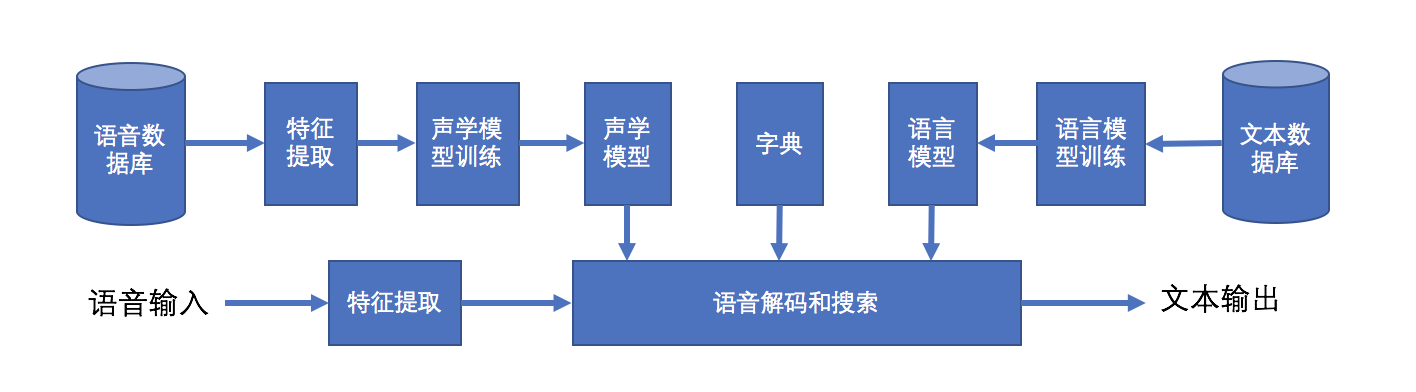
\includegraphics[width=0.9\textwidth]{img/chapter_lm/asr-pipeline2.png}
		\caption{语音音识别基本流程}
		\label{pic:asr}
	\end{center}
\end{figure}

自动语音识别(Automatic Speech Recognition,ASR)是一种将人的语音转换为文本的技术,它是目前很多互联网产品如语音助手,语音搜索引擎等中必不可少的一部分。
图~\ref{pic:asr}给出了常见的语音识别系统的基本工作流程。其中基本可以分为以下几个模块:
\begin{itemize}
    \item 数据预处理: 典型的预处理包含静音处理(Voice Activity Detection,VAD)等,用于去除其中的静音片段。
	\item 特征提取:将声音转换成包含声音信息的多维向量,常见的有MFCC等。
	\item 声学模型:主要是通过语音数据训练得到,其输出是音素等信息。
	\item 词典:字/词和音素之间的对应关系。
	\item 语言模型:也就是上文提到的语言模型部分,主要用于评估字或者词序列的概率。
\end{itemize}

\noindent 语音系统首先将语音信号做特征提取工作,转化成诸如MFCC等特征来表示,然后使用语言模型和声学模型来解码,解码过程会产生很多候选(Candidates),最终最优的候选会被输出成为最终的结果。语言模型是其中很重要的一部分,它用于从根据语言统计规律评估声学模型给出的句子序列候选的概率,决定了最终输出的结果。 
\section{主题模型}

\subsection{基本概念}
主题模型 (Topic Models) 是近些年来非常重要的一项技术,它被广泛应用于工业和学术界。在主题模型中,我们一般用$d$来表示要分析的文档,例如一篇文章或者一个网页等,而一个文档$d$通常由一系列词$(w_1, w_2, ..., w_n)$组成, 其中$w_n$ 是文档中的第$n$个词。多份文档共同构成了我们要分析的语料集,我们用$\mathcal{D}$来表示,$\mathcal{D}=(d_1, d_2, ..., d_m)$组成,其中$d_m$ 是语料库中的第$m$个文档。主题一般用$z$来表示,它由一些词组成,同时也有该词在这个主题下的概率。
主题模型泛指由一类可以从语料库中抽取主题并利用这些主题表示文档的模型,常见的主题模型有PLSA,LDA,以及各种LDA的变种,例如SentenceLDA等。在熟悉了这些基本概念之后,我们通过一种常见的主题模型Latent Diriclet Allocation (LDA)来认识主题模型。




\subsection{常见的主题模型:LDA}

2003年Blei等人在《Latent Dirichlet Allocation》~\cite{blei2003latent} 一文中提出了LDA模型。
如图\ref{pic:lda}所示,其中空心节点表示隐藏变量,实心变量表示客观测变量,整个模型具有K个主题,M个文档和N个词。
LDA将文档的主题分布$P(z|d)$看做随机变量$\theta$,并且假设$\theta$从一个狄利克雷先验中产生。
同时,由于训练数据之外的文档对应的主题分布$\theta$可以从上述狄利克雷分布中产生,训练数据之外的文档的$\theta$可以更自然地进行计算。

\begin{figure}[htb]
	\begin{center}
		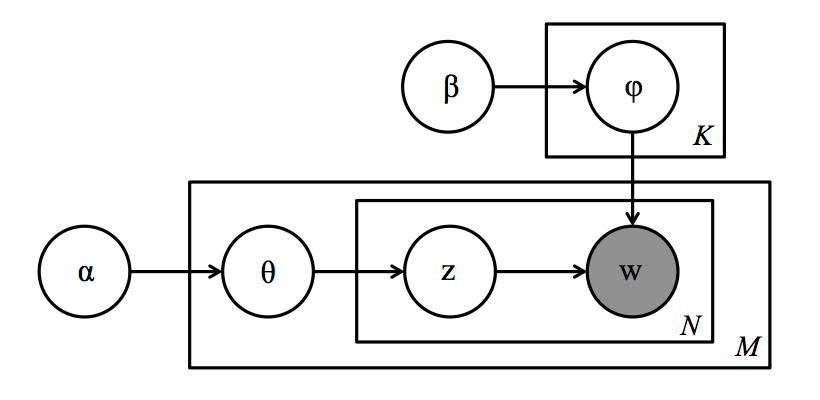
\includegraphics[width=0.8\textwidth]{img/chapter_lm/lda.png}
		\caption{LDA图模型}
		\label{pic:lda}
	\end{center}
\end{figure}

\subsection{主题模型在语音识别中的应用: 语言模型适配}

\begin{figure}[htb]
	\begin{center}
		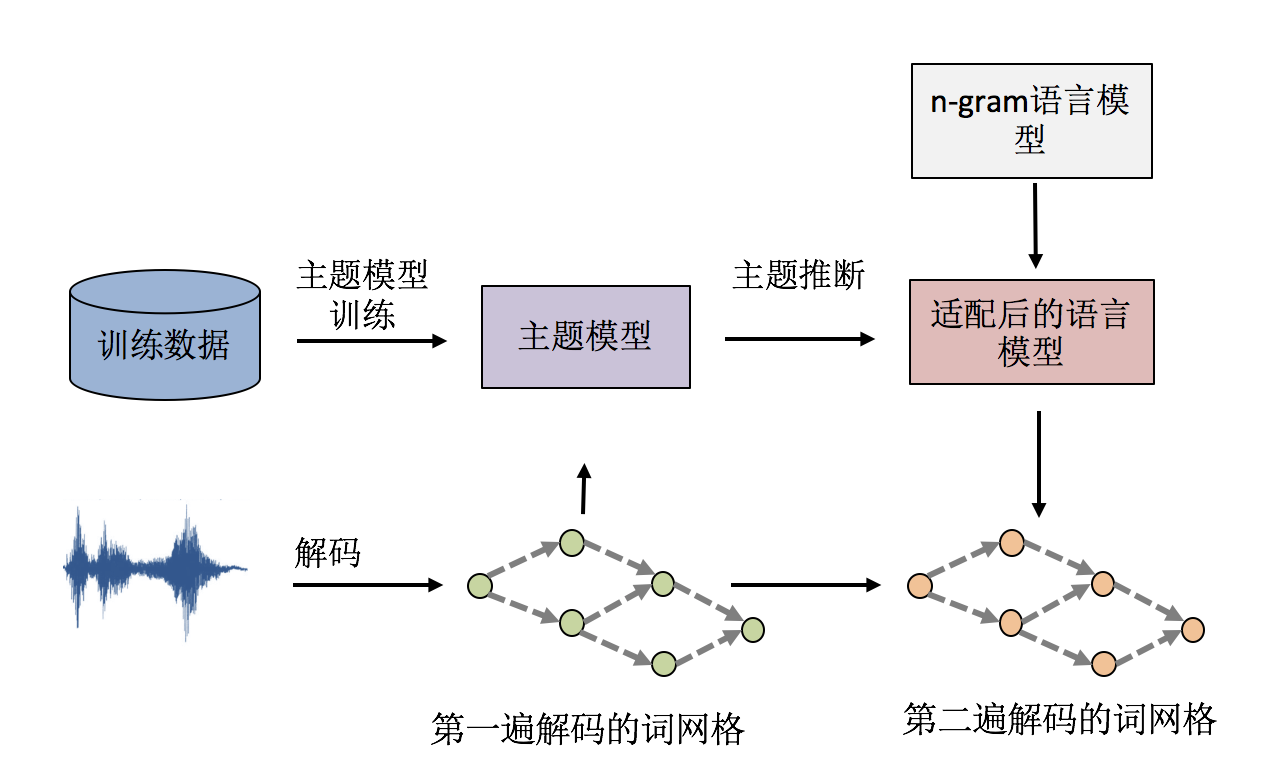
\includegraphics[width=0.8\textwidth]{img/chapter_lm/lma2.png}
		\caption{语言模型适配}
		\label{pic:lma}
	\end{center}
\end{figure}

语音识别系统中一个常见的问题就是,我们训练语言模型的语料和它实际线上应用的语料之间存在不一致,这种情况下,除了重新训练模型,有一种代价更小的方法就是语言模型适配(Language Model Adaptation)。
语言模型适配指的是用实际应用的语料相关的信息,对语言模型做适配。图~\ref{pic:lma}给出了其常见的工作流程,采用预先训练好的主题模型,我们对语音识别系统第一遍识别出来的词网格
(Word Lattice)做主题推断,可以发现其语义级别的内容,同时它也可以作为一个unigram的语言模型$P_{LDA}(w|\theta_d)=\sum_{k \in K} \varphi_{kw} \theta_{dk}$,对之前的n-gram语言模型就行适配:
\begin{equation}
\begin{aligned}
P_{d}(w|C) = \lambda P_{LDA}(w|\theta_d) + (1-\lambda) P_{n-gram \ LM}(w|C)
\end{aligned}
\label{eq:hb_model}
\end{equation}
其中$C$代表当前词$w$的上下文,$\lambda$是一个权重参数,$P_{n-gram\ LM}(w|C)$是基础的ngram语言模型给出来的评估分数。这个新适配过的语言模型,可以用于语音识别系统,重新解码出新的词网格以及最终的结果。
